\documentclass[12pt,a4paper]{article}

\usepackage[utf8]{inputenc}
\usepackage[T1]{fontenc}
\usepackage[french]{babel}

\usepackage{styles/couleurs}
\usepackage{styles/mise_en_page}
\usepackage{styles/boites}
\usepackage{styles/maths}
\usepackage{styles/figures}

\usepackage{amsmath}
\usepackage{amssymb}
\usepackage{array}
\usepackage{tabularx}
\usepackage{graphicx}
\usepackage[most]{tcolorbox}

% =========================================================
% MISE EN PAGE
% =========================================================

\geometry{
  top=1.25cm,
  bottom=1.15cm,
  left=1.35cm,
  right=1.35cm
}

\setlength{\parindent}{0pt}
\setlength{\parskip}{0pt}
\setlength{\tabcolsep}{3pt}

\setlength{\abovedisplayskip}{3pt}
\setlength{\belowdisplayskip}{3pt}
\setlength{\abovedisplayshortskip}{2pt}
\setlength{\belowdisplayshortskip}{2pt}

\begin{document}

% =========================================================
% TITRE
% =========================================================

\begin{center}
{\sffamily\Large\bfseries Théorème de Pythagore : rédiger}
\end{center}

\vspace{0.15em}

% =========================================================
% ÉTAPE 1
% =========================================================

{\sffamily\large\bfseries\underline{Étape 1 : Maîtriser la formule}}

\smallskip

Complète le tableau en utilisant la figure.

\medskip

\noindent
\begin{minipage}[t]{0.59\linewidth}
\vspace{0pt}

\footnotesize

\renewcommand{\arraystretch}{1.12}

\begin{tabularx}{\linewidth}{
|>{\centering\arraybackslash}p{1.35cm}|
 >{\centering\arraybackslash}p{1.8cm}|
 >{\centering\arraybackslash}X|
}
\hline
\textbf{Triangle}
&
\textbf{Rectangle en}
&
\textbf{Égalité de Pythagore}
\\
\hline

ACI & C & $AI^2=AC^2+CI^2$ \\ \hline
DEI & & \\ \hline
CHI & & \\ \hline
HIM & & \\ \hline
JLM & & \\ \hline
JLK & & \\ \hline
JKM & & \\ \hline
HJK & & \\ \hline
GFH & & \\ \hline
GFB & & \\ \hline
BGH & & \\ \hline
BCH & & \\ \hline

\end{tabularx}

\end{minipage}
\hfill
\begin{minipage}[t]{0.38\linewidth}
\vspace{0pt}

\centering

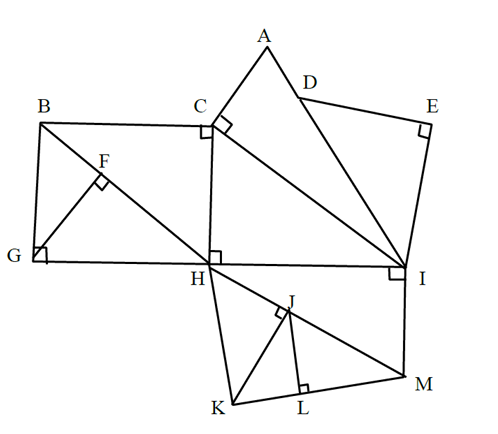
\includegraphics[
  width=\linewidth,
  height=7.2cm,
  keepaspectratio
]{images/ap pythagore rédaction.png}

\end{minipage}

\vspace{0.45em}

% =========================================================
% ÉTAPE 2
% =========================================================

{\sffamily\large\bfseries\underline{Étape 2 : Maîtriser les éléments de langage}}

\smallskip

On considère le triangle \(ACI\) de l'étape 1 avec
\(AC=3\) cm et \(CI=4\) cm.

\smallskip

Dans la liste ci-dessous, \textbf{surligne les phrases que tu garderais}
pour rédiger correctement la solution.

\medskip

\begin{tcolorbox}[
  enhanced,
  colback=white,
  colframe=black!55,
  boxrule=0.5pt,
  arc=0mm,
  left=3mm,
  right=3mm,
  top=1.5mm,
  bottom=1.5mm
]

\small

\begin{minipage}[t]{0.49\linewidth}

1) Le triangle est rectangle

\smallskip

2) D'après Pythagore

\smallskip

3) On sait que \(AI=5\) cm donc
\(AI^2=AC^2+CI^2\)

\smallskip

4) \(AI^2=\sqrt{25}\)

\smallskip

5) \(AI^2=3^2+4^2\)

\smallskip

6) D'après le théorème de Pythagore

\smallskip

7) Le triangle \(ACI\) est un rectangle

\smallskip

8) On utilise le thm de Pithagaure

\end{minipage}
\hfill
\begin{minipage}[t]{0.49\linewidth}

9) \(AI=\sqrt{25}\)

\smallskip

10) \(AI^2=3\times3+4\times4\)

\smallskip

11) Donc : \(AI=5\) cm

\smallskip

12) \(AI^2=9+16\)

\smallskip

13) \(ACI\) est un triangle rectangle en \(C\)

\smallskip

14) \(AI^2=25\)

\smallskip

15) \(AI^2=AC^2+CI^2\)

\end{minipage}

\end{tcolorbox}

\vspace{0.35em}

% =========================================================
% RECONSTRUIRE LA RÉDACTION
% =========================================================

\begin{tcolorbox}[
  enhanced,
  colback=ActionC!5,
  colframe=ActionC!55,
  boxrule=0.6pt,
  arc=1.5mm,
  left=3mm,
  right=3mm,
  top=1.3mm,
  bottom=1.3mm
]

{\sffamily\bfseries\color{ActionC}
Remets les phrases dans l'ordre.}

\smallskip

Écris les \textbf{numéros des phrases choisies} pour reconstruire
une rédaction complète.

\medskip

\begin{center}
\boxed{\phantom{13}}
\;\longrightarrow\;
\boxed{\phantom{13}}
\;\longrightarrow\;
\boxed{\phantom{13}}
\;\longrightarrow\;
\boxed{\phantom{13}}
\;\longrightarrow\;
\boxed{\phantom{13}}
\;\longrightarrow\;
\boxed{\phantom{13}}
\;\longrightarrow\;
\boxed{\phantom{13}}
\;\longrightarrow\;
\boxed{\phantom{13}}
\end{center}

\end{tcolorbox}

% Correction possible :
% 13 -> 6 -> 15 -> 5 -> 12 -> 14 -> 9 -> 11
% La phrase 10 peut remplacer la phrase 5.

\vspace{0.45em}

% =========================================================
% ÉTAPE 3
% =========================================================

{\sffamily\large\bfseries\underline{Étape 3 : Synthèse}}

\smallskip

Sur ton cahier, rédige en utilisant ce que tu as appris
la solution de l'exercice suivant.

\medskip

\begin{tcolorbox}[
  enhanced,
  colback=NeutreBg,
  colframe=NeutreC!45,
  boxrule=0.5pt,
  arc=1.5mm,
  left=3mm,
  right=3mm,
  top=1.4mm,
  bottom=1.4mm
]

\(IJK\) est un triangle rectangle en \(K\) tel que :

\[
IK=7\text{ cm}
\qquad\text{et}\qquad
JK=2{,}4\text{ cm}.
\]

\textbf{Calculer la longueur \(IJ\).}

\end{tcolorbox}

\end{document}